% Functional specification for ProfiSnort
\documentclass[listof=totoc,a4paper]{scrreprt}

\usepackage[german]{babel}
\usepackage[utf8]{inputenc}
\usepackage[T1]{fontenc}
\usepackage{ae}
\usepackage[bookmarks,bookmarksnumbered]{hyperref}
\usepackage{csquotes}
\usepackage{longtable}
\usepackage{enumitem, hyperref}
\usepackage{graphicx}

\usepackage[ampersand]{easylist}
\usepackage{xcolor}

\usepackage[toc,acronym]{glossaries}
\makeglossaries

\setuptoc{toc}{totoc}

\usepackage{xparse}
\DeclareDocumentCommand{\newdualentry}{ O{} O{} m m m m } {
  \newglossaryentry{gls-#3}{name={#5},text={#5\glsadd{#3}},
    description={#6},#1
  }
  \makeglossaries
  \newacronym[see={[Glossary:]{gls-#3}},#2]{#3}{#4}{#5\glsadd{gls-#3}}
}

\renewcommand*{\glstextformat}[1]{\textcolor{black}{#1}}

\hypersetup{
	backref,
    colorlinks,
    linkcolor=[RGB]{0,153,84},
    citecolor={blue!40!black},
    urlcolor={blue!70!black},
    linktocpage=true
}

\makeatletter
\def\namedlabel#1#2{\begingroup
    #2%
    \def\@currentlabel{#2}%
    \phantomsection\label{#1}\endgroup
}
\makeatother

\newcounter{savepage}

\newcommand{\sppname}{spp\_profinet}
\newcommand{\programname}{TruffleHog}


\loadglsentries{../../global_tex_files/glossary}


\begin{document}

\title{\programname \ \& \sppname \ -- Entwurf}
\author{
    Brendl, Julian
    \texttt{julian.brendl@student.kit.edu}
    \and
    Diez, Maximilian
    \texttt{maximilian.diez@student.kit.edu}
    \and
    Giraud, Mark
    \texttt{mark.giraud@student.kit.edu}
    \and
    Hermes, Jan
    \texttt{jan.hermes@student.kit.edu}
    \and
    Höhler, Dimitri
    \texttt{dimitri.hoehler@student.kit.edu}
    \and
    Kiechle, Valentin
    \texttt{valentin.kiechle@student.kit.edu}
}

\titlehead{
\includegraphics[width=150pt]{images/title.png}}

\maketitle

\pagenumbering{Roman}
\setcounter{page}{2}

\newpage
\tableofcontents
\newpage
\listoffigures

\printglossary[title=Abkürzungsverzeichnis,toctitle=Abkürzungsverzeichnis,type=acronym]

\clearpage
\setcounter{savepage}{\arabic{page}}
\pagenumbering{arabic}
\setcounter{page}{\thesavepage}

\chapter{Einleitung}
Dieses Dokument dient der genaueren Beschreibung und Dokumentation des Entwurfs zum Visualisierungstool \gls{programname}, dessen Hauptaufgabe die Darstellung des Netzwerkverkehrs eines \gls{profinet}-Systems ist. Des Weiteren wird der im \gls{ids} \gls{snort} eingebaute \gls{praeprozessor} \gls{sppname} und die genaue Funktionsweise der \gls{ipc} zu \gls{programname} erläutert.\newline
\newline


Das Design von \gls{programname} baut auf dem klassischen \gls{mvc} auf und erweitert diesen Entwurf zu einem \gls{mvp} mit zusätzlicher Funktionalität. Das heisst, dass der Controller aufgeteilt wurde in zwei selbständige Packages. Zum Einen das Service-Package. Dabei handelt es sich um entkoppelte, selbstlaufende Routinen, welche fast die gesamte Logik des Programms ausmachen. Sie werden einmal initialisiert und laufen dann solange \gls{programname} läuft. Zum Andern gibt es den Presenter. Dieser erfüllt seine Hauptaufgabe bei Programmstart. Er instanziiert alle für den Programmablauf benötigten Klassen. Außerdem erstellt er sämtiche nötigen Referenzen, übergibt diese, und startet jeden selbständigen Thread wie zum Beispiel die Services. Danach wird der Presenter nicht mehr benötigt.

Der Entwurf von \gls{programname} baut auf das klassische \gls{mvc} Design auf, welches bereits im Pflichtenheft präsentiert wurde (siehe Abbildung~\ref{fig:old_arch_diagram}). Das erweiterte \gls{mvc} Modell in Abbildung~\ref{fig:arch_diagram} zeigt, dass der Aufbau sich um folgende Bestandteile

MODEL:
Wie im traditionellen \gls{mvc} Muster dient das Model ausschließlich zur Speicherung von Daten in geeigneten Datenstrukturen. Im Fall von \gls{programname} umfasst dies den Graphen (siehe Kapitel~\ref{subsubsec:graph}.) und die Programmeinstellungen.

VIEW:
Auch der View unterscheidet sich kaum von der ursprünglichen Funktionalität. Er dient weiterhin dazu, dem Benutzer eine Plattform zur Interaktion mit dem Programm zu bieten. Ein wesentlicher Unterschied zum ursprünglichen Aufbau ist hierbei jedoch, dass der View nur spezifische Interaktionen (siehe INTERACTIONS) kennt und ausführen kann. Wobei der View keine Kenntnis über die hinter der Aktion stehende Logik hat.

INTERACTIONS:
Wie bereits im vorherigen Absatz beschrieben, dienen Interaktionen dem View als 

COMMANDS:
Kommandos sind neben dem SERVICE Package die eigentlichen 

PRESENTER:
Im Presenter wird die gesamte Aufbauarbeit geleistet. Kommandos werden mit bestimmten Interaktionen gelinkt, grafische Oberflächen werden instanziiert und vorbereitet und das Modell.
Zusätzlich kümmert sich der Presenter darum, dass sämtliche Service Routinen gestartet werden 


Der Presenter ist dafür verantwortlich, dass sämtliche Klassen instanziiert werden 

Wie  in 


\begin{figure}[H]
  \centering
  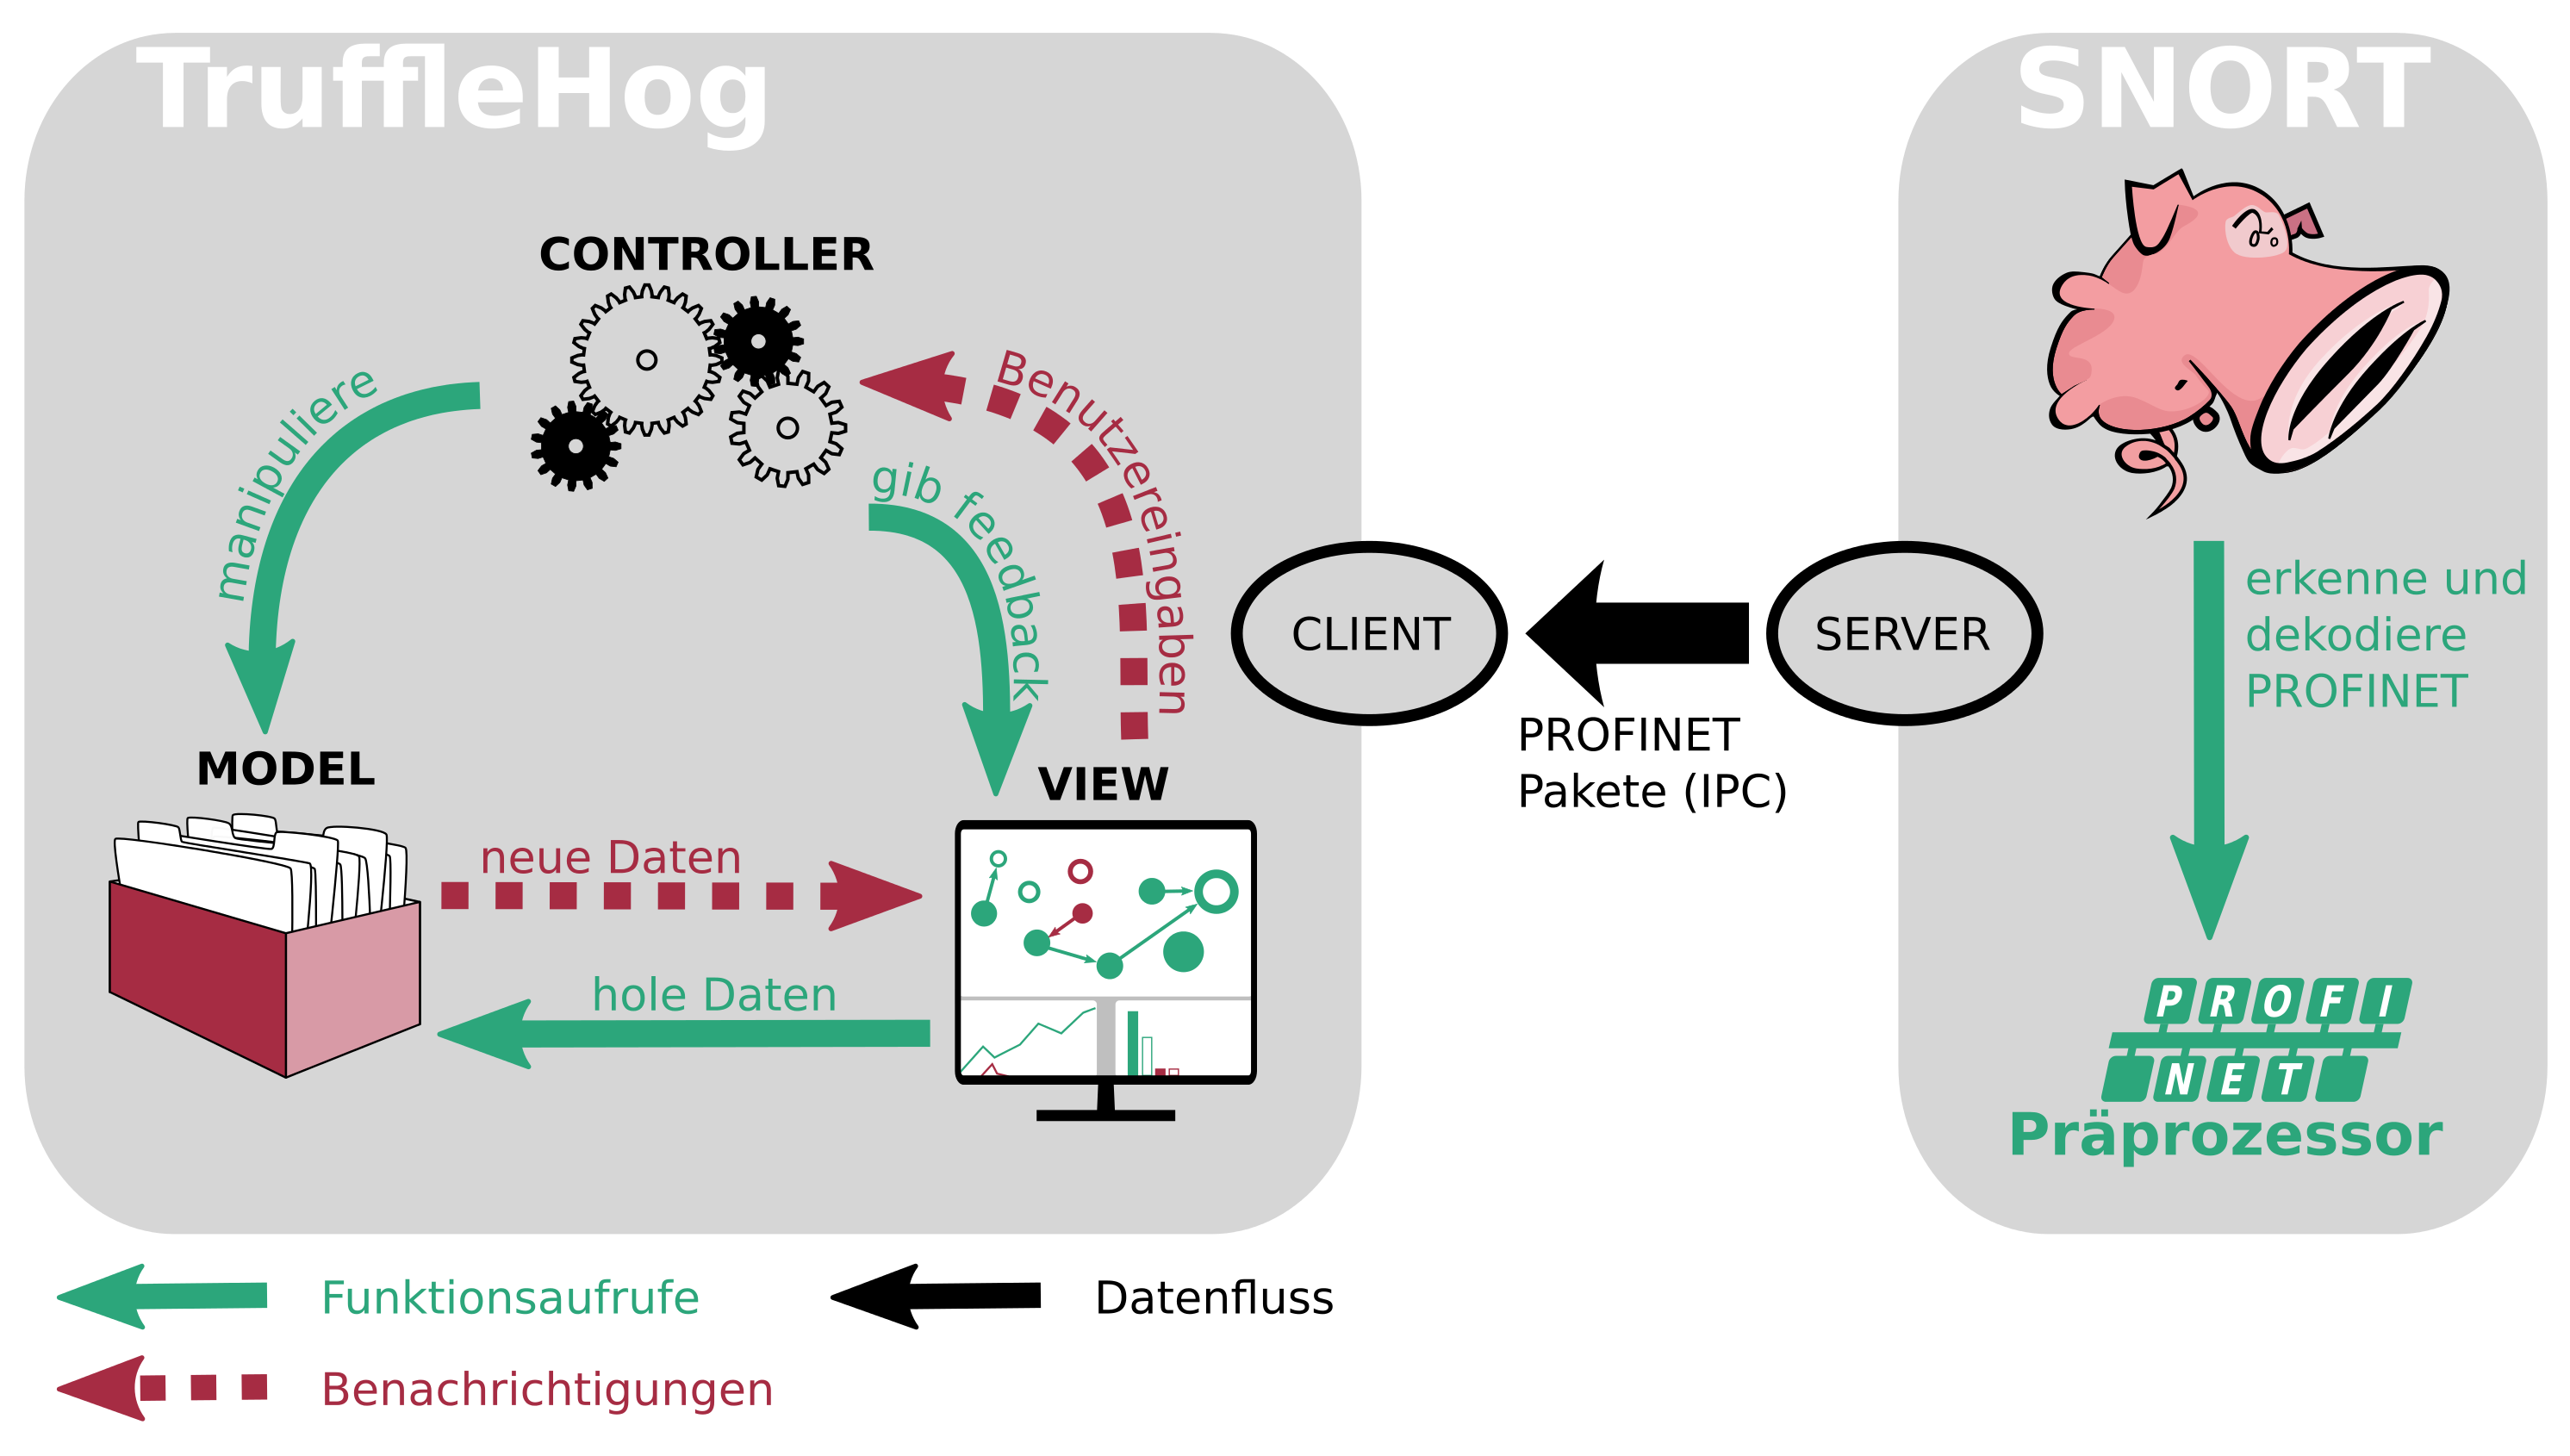
\includegraphics[width=0.8\textwidth]{../diagramimages/praesentationsmodel.png}
  \caption[Urspr''ungliche Architektur''ubersicht]{Urspr''ungliche Architektur''ubersicht}
  \medskip
  Ursprünglicher Aufbau der Programme aus dem Pflichtenheft
\end{figure} 

\begin{figure}[H]
  \centering
  \includegraphics[width=0.8\textwidth]{../diagramimages/arch_diagram_mvp_single.pdf}
  \caption[Erweiterte Architekturu''bersicht]{Erweiterte Architekturu''bersicht}
  \medskip
  Erweiterte Strukturierung des Programms nach dem \gls{mvp}
\end{figure} 

\section{Architekturbeschreibung}
Im Groben gehalten funktioniert der Daten- und Befehlsfluss im Trufflehog-Entwurf
wie im klassischen MVC, der Presenter aktiviert Services, welche das Model basierend
auf dem empfangenen Netzwerkverkehr verändert und das View aktualisiert sich am Model.
Da viele Threads im Programm parallel durchlaufen aber dennoch kommunizieren müssen,
verlassen wir uns an einigen Stellen auf das \gls{observerpattern} mit einer
Multi-Thread kompatiblen Datenstruktur.\newline
\newline


\chapter{Klassendokumentation}

\section{Service}

\subsection{TruffleReceiver}

\begin{figure}[H]
    \centering
    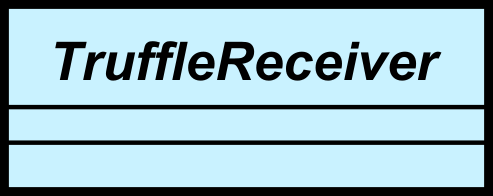
\includegraphics{../diagramimages/TruffleReceiver.png}
    \caption[Klasse TruffleReceiver]{Klasse TruffleReceiver}
    \medskip
    Diese Klasse empfängt ganz tolle Truffles und so ein zeug bla bla.
\end{figure}

\subsubsection*{Attribute}

\begin{easylist}[itemize]

    & Attribut 1

    & Attribut 2

\end{easylist}

\subsubsection*{Methoden}

\begin{easylist}[itemize]

    & Methode 1

    & Methode 2

\end{easylist}

\subsection{Truffle}

\begin{figure}[H]
    \centering
    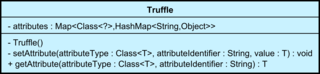
\includegraphics{../diagramimages/Truffle.png}
    \caption[Klasse Truffle]{Klasse Truffle}
    \medskip
    Klasse, welches empfangenen Datenverkehr modelliert.
\end{figure}

\subsubsection*{Attribute}

\begin{easylist}[itemize]

    & Attribut 1

    & Attribut 2

\end{easylist}

\subsubsection*{Methoden}

\begin{easylist}[itemize]

    & Methode 1

    & Methode 2

\end{easylist}

\subsection{MessageQueueReceiver}

\begin{figure}[H]
    \centering
    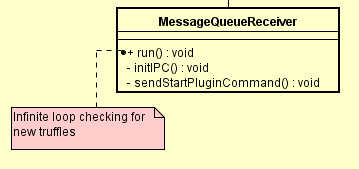
\includegraphics{../diagramimages/MessageQueueReceiver.png}
    \caption[Klasse MessageQueueRceceiver]{Klasse MessageQueueReceiver}
    \medskip
    Die konkrete Empfangsklasse für Truffles.
\end{figure}

\subsubsection*{Attribute}

\begin{easylist}[itemize]

    & Attribut 1

    & Attribut 2

\end{easylist}

\subsubsection*{Methoden}

\begin{easylist}[itemize]

    & Methode 1

    & Methode 2

\end{easylist}

\section{Presenter}

\section{Commands}

\section{Model}

\section{View}

\section{Interactors}

\section{Util}

\chapter{Sequenzdiagramme}



\chapter{Ressourcen}
\section{Dateien und Strukturen}
Im Folgenden ist das Datenhaltungsverzeichnis von \gls{programname} visualisiert. Alle persistenten, das heißt einen Neustart des Programms überdauernden Daten sind in Dateien in Unterordnern des Ordners \texttt{data} gespeichert.  
\begin{figure}[htb]
  \centering
\begin{verbatim}
.
`-- data
    |-- config
    |   |-- filtermenu_en.properties
    |   |-- graphwindow_en.properties
    |   |-- logwindow_en.properties
    |   |-- notificationview_en.properties
    |   |-- settingsmenu_en.properties
    |   `-- statistics_en.properties
    |-- log
    |   `-- trufflehog.log
    |-- replay_log
    |   |-- graph_TIMESTAMP2.trufflesnapshot
    |   `-- graph_TIMESTAMP.trufflesnapshot
    `-- truffle_data_log
        |-- nodeA.xml
        `-- nodeB.xml
\end{verbatim}
  \caption[Ordner- und Dateiestruktur von \gls{programname}]{Ordner- und Dateiestruktur von \gls{programname}}
\end{figure}
\begin{itemize}
\item[\texttt{config}] Einen Neustart des Programms überdauernde Informationen über die visuellen Teile des Programms und Speicherung sprachlicher Lokalisierungen. 
\item[\texttt{log}] Zentrale Logdatei des Programms. 
\item[\texttt{replay\_log}] Gesamtzustand des Graphen zu einem Zeitpunkt plus Veränderungen über eine gewisse Zeitspanne. 
\item[\texttt{truffle\_data\_log}] Logdatei zu jedem Knoten mit zeilenweiser Auflistung der verarbeiteten Truffles.
\end{itemize}

\section{Externe Bibliotheken}
\subsection{Java Universal Network/Graph Framework}
Die Bibliothek Java Universal Network/Graph Framework (JUNG) ist eine seit 2003 entwickelte Java-Bibliothek zur Speicherung, Visualisierung und zu Rechnen mit Graphen und graphähnlichen Strukturen. Sie ist modular aufgebaut und kapselt alle oben genannten Funktionen in verschiedenen Bibliotheksteilen. Außerdem bietet sie erweiterte Funktionalitäten wie verschiedene Anordnungsalgorithmen, diverse Annotationsmöglichkeiten der Visualisierung und Algorithmen zur Graphanalyse. 
\subsubsection{Motivation}
JUNG hat alle für \gls{programname} relevanten Funktionen einer Graphbibliothek und bietet zudem folgende Vorteile gegenüber vergleichbaren Bibliotheken. 

Für sämtliche Klassen der Bibliothek werden Interfaces bereitgestellt. Dies bedeutet, dass ohne Kompatibilitätsverlust neue Funktionen eingebunden werden können. 

Die kritischen Komponenten, also die Visualisierung, Datenhaltung und Graphlogik ist in JUNG modular voneinander abgegrenzt. Dies ermöglicht die perfekte Einbindung in das \gls{mvc}-Konzept von \gls{programname}. Viele andere Graphbibliotheken koppeln Datenhaltung und Visualisierung und würden somit keine klare Trennung des \gls{mvc} ermöglichen. 

JUNG ist als sehr stabile und verlässliche Bibliothek bekannt, die Wert auf Kompatibilität und weitgehende Fehlerfreiheit legt. 

Die Vorteile davon, dass JUNG eine Open Source-Projekt ist verstehen sich von selbst. 

\subsubsection{Verwendungsbeschreibung}




\chapter{Klassenverzeichnis}

\appendix

\printglossary[title=Glossar,toctitle=Glossar]

\end{document}
